\chapter{Introduction}

Web-based applications have grown in popularity in recent years. From the early days of simple web applets to current full-blown programs, their codebase's complexity and size grow rapidly. Due to the design of most browsers, programmers have to choose JavaScript or its dialects to implement them. This approach is quite successful; however, it still leaves several problems unsolved. First, JavaScript is a scripting language and employs many dynamic features that prevent backend runtime environment from efficient execution, such as dynamic typing. Additionally, when porting existing applications to JavaScript, especially those with a large codebase where manually translating source code line-by-line is not feasible, a nontrivial source-to-source compiler is needed due to the structural difference between native binaries and JavaScript source codes. To address these problems, the WebAssembly working group is established in 2017, and purpose a new standard for distributing applications over the Internet. WebAssembly focuses on safety, performance, portability and module compactness. These properties also make it an interesting target for static execution, enabling sandboxed applications outside of browsers. To this end, the WebAssembly community further design the WebAssembly System Interface (WASI), which provides a standardized interface for WebAssembly modules to access native features such as the file system.

WebAssembly is also an evolving language. Although the WebAssembly community has published the minimum viable product (MVP) WebAssembly, the community is still actively proposing and experimenting with new language features, such as exception handling and garbage collection. These additional language features are purposed in language extension proposals that modify the current WebAssembly specification syntactically and semantically. Thus, a well-designed WebAssembly runtime environment system should be modular and extensible, leaving space for future design changes.

\section{Contribution}

\begin{figure}
    \centering
    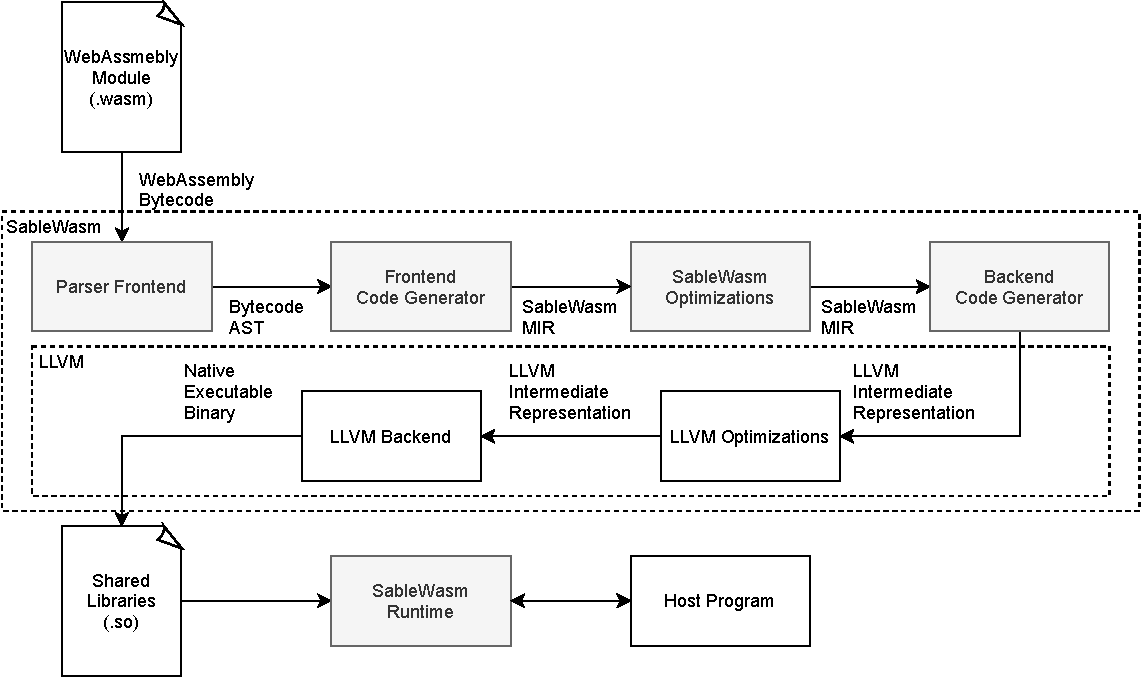
\includegraphics[width=\textwidth]{Images/design}
    \caption{The SableWasm compiler and runtime}
    \label{fig:design}
\end{figure}

This thesis aims to design and implement a runtime environment that enables
WebAssembly to run outside of the browser. To this end, this thesis makes three
major contributions. Figure~\ref{fig:design} illustrates SableWasm compiler and
runtime system. We mark our contributions in this thesis as shaded boxes in the
figure.

\paragraph{Implementing a WebAssembly runtime system}
Our first contribution is a standalone WebAssembly runtime environment with
support for \emph{WebAssembly System Interface} (WASI). We first start by
implementing a custom extensible parser frontend for WebAssembly binary format.
We then define a middle-level representation for SableWasm. SableWasm MIR is a
register-based control flow graph representation of the program, while, on the
other hand, WebAssembly operates over a stack-based virtual machine. Hence,
translating between them is nontrivial. Therefore, we design and implement a
frontend code generator that lowers WebAssembly bytecode into SableWasm MIR.
SableWasm MIR plays a critical role in the SableWasm system. First, it provides
a middle ground where we implement an extensible and straightforward
optimization framework. With the help of the framework, we experiment several
analyses and optimizations on SableWasm MIR. Second, SableWasm MIR also
separates the frontend from the backend. Currently, we implement an
ahead-of-time (AOT) compiler backend using the LLVM compiler infrastructure.
However, there are several challenges when lowering SableWasm MIR into LLVM
intermediate representation. For example, SableWasm MIR, similar to WebAssembly
bytecode, utilizes several abstract high-level concepts such as linear memory
and indirect function call. These operations cannot be trivially mapped to LLVM
instructions and requires runtime library support. Hence, the last component of
SableWasm is a runtime library that provides builtin runtime functions for the
generated modules and defines an easy-to-use interface for the host system.

\paragraph{Adding support for WebAssembly extensions}
Our second contribution in this thesis is to experiment and adopt several
in-progress WebAssembly language extensions. SableWasm is designed to be
extensible and currently implements four post-MVP WebAssembly features. The
most interesting one among them is perhaps the fixed-width SIMD operation
extension which introduces one additional value type and approximately 240
new instructions to the specification. As we have discussed earlier in this
section, SableWasm MIR provides a middle ground where we perform optimization
on the program. Therefore, we would like to keep the size of the SableWasm MIR
instruction set simple. To achieve this goal, we carefully design a set of
reduction patterns in the frontend code generator that significantly reduce the
number of instructions needed. We also generalize our backend code generator
that targets LLVM by emitting corresponding vector operation instructions.

\paragraph{Evaluating system performance}
Our last contribution in this thesis is to investigate how SableWasm performs
and the factors that affect the performance. Here we focus on three research
questions: First, how does SableWasm perform comparing to other existing
WebAssembly runtime implementations? Second, does optimization over the input
WebAssembly modules affect SableWasm's overall performance? Finally, does the
SIMD operation extension bring performance improvement to the system? To answer
these questions, we perform benchmarks against three well-known benchmark
suites, Polybench \cite{polybench}, Ostrich \cite{ostrich}, and NPB \cite{npb}.
We also exam generated LLVM intermediate representations in SableWasm to search
for factors contributing to the slow down in the system.

\section{Thesis outline}

This thesis consists of eight chapters in total, including the introduction
chapter. Chapter 2 discusses the background information that helps the
understanding rest of the thesis. It first presents the motivation for
WebAssembly and WebAssembly System Interface (WASI), followed by a brief
overview of the LLVM intermediate representation. Chapter 3 to chapter 5
discusses the design of implementation of the SableWasm system. Chapter 3 starts
with presenting the custom extensible and efficient parser frontend for
WebAssembly binary format. Chapter 4 continues the discussion of SableWasm by
describing SableWasm MIR, including the code generating strategies used when
lowering WebAssembly bytecode to SableWasm MIR and the optimization framework.
Chapter 4 also presents several optimization passes we experimented with the
framework, such as control flow graph simplification and type inference.
Chapter 5 illustrates the last component of SableWasm, the LLVM backend and the
runtime support library. In chapter 6, we investigate the performance of
SableWasm by presenting benchmark results and discussing several possible
theories for the slowdown. Finally, chapter 7 discusses related work and
chapter 8 presents our conclusion along with future work.